%%%%%%%%%%%%%%%%%%%%%%%%%%%%%%%%%%%%%%
% Multiplicative domain poster
% Created by Nathaniel Johnston
% August 2009
% http://www.nathanieljohnston.com/2009/08/latex-poster-template/
%%%%%%%%%%%%%%%%%%%%%%%%%%%%%%%%%%%%%%

\documentclass[final]{beamer}
\usepackage[scale=1.24]{beamerposter}
\usepackage{graphicx}			% allows us to import images

%-----------------------------------------------------------
% Custom commands that I use frequently
%-----------------------------------------------------------

\newcommand{\bb}[1]{\mathbb{#1}}
\newcommand{\cl}[1]{\mathcal{#1}}
\newcommand{\fA}{\mathfrak{A}}
\newcommand{\fB}{\mathfrak{B}}
\newcommand{\Tr}{{\rm Tr}}
\newtheorem{thm}{Theorem}

%-----------------------------------------------------------
% Define the column width and poster size
% To set effective sepwid, onecolwid and twocolwid values, first choose how many columns you want and how much separation you want between columns
% The separation I chose is 0.024 and I want 4 columns
% Then set onecolwid to be (1-(4+1)*0.024)/4 = 0.22
% Set twocolwid to be 2*onecolwid + sepwid = 0.464
%-----------------------------------------------------------

\newlength{\sepwid}
\newlength{\onecolwid}
\newlength{\twocolwid}
\setlength{\paperwidth}{1189mm}
\setlength{\paperheight}{841mm}
\setlength{\sepwid}{0.024\paperwidth}
\setlength{\onecolwid}{0.22\paperwidth}
\setlength{\twocolwid}{0.464\paperwidth}
\setlength{\topmargin}{-0.5in}
\usetheme{confposter}
\usepackage{exscale}
\usepackage{graphicx}
\usepackage{subcaption}
\usepackage{array}
\usepackage{booktabs}% http://ctan.org/pkg/booktabs

\newcommand{\tabitem}{~~\llap{\textbullet}~~}
\def\LW{\dimexpr.2\linewidth-.0em}


%-----------------------------------------------------------
% The next part fixes a problem with figure numbering. Thanks Nishan!
% When including a figure in your poster, be sure that the commands are typed in the following order:
% \begin{figure}
% \includegraphics[...]{...}
% \caption{...}
% \end{figure}
% That is, put the \caption after the \includegraphics
%-----------------------------------------------------------

\usecaptiontemplate{
\small
\structure{\insertcaptionname~\insertcaptionnumber:}
\insertcaption}

%-----------------------------------------------------------
% Define colours (see beamerthemeconfposter.sty to change these colour definitions)
%-----------------------------------------------------------

\setbeamercolor{block title}{fg=ngreen,bg=white}
\setbeamercolor{block body}{fg=black,bg=white}
\setbeamercolor{block alerted title}{fg=white,bg=dblue!70}
%\setbeamercolor{block alerted body}{fg=black,bg=dblue!10}
\setbeamercolor{block alerted body}{fg=black,bg=white}


%-----------------------------------------------------------
% Name and authors of poster/paper/research
%-----------------------------------------------------------

%\title{\parbox[c]{38in}{Lineage diversification in the genus \textit{Solanum }L. (Solanaceae)}
%\parbox[c]{5in{\includegraphics[width=5in]{./logos/ICL_logo.PNG}}\\ \includegraphics[width=5in]{./logos/ICL_logo.PNG}}}
\title{Plant functional diversity and the biogeography of biomes in North and South America}
\author{Susy Echeverr\'ia-Londo\~no$^{1*}$, Brian J. Enquist$^{2}$, Danilo M. Neves$^{2}$, Cyrille Violle$^{3}$ \& Andrew J, Kerkhoff$^{1}$}
\institute{\small (1) Department of Biology, Kenyon College, Gambier, Ohio, USA; (2) Department of Ecology and Evolutionary Biology, University of Arizona, Tucson, Arizona, USA; (3) Centre d'Ecologie Fonctionnelle et Evolutive (UMR 5175), CNRS, Universit\'e de Montpellier, Universit\'e Paul Val\'ery, Montpellier, France \\ *echeverrialondono1@kenyon.edu}

%-----------------------------------------------------------
% Start the poster itself
%-----------------------------------------------------------
% The \rmfamily command is used frequently throughout the poster to force a serif font to be used for the body text
% Serif font is better for small text, sans-serif font is better for headers (for readability reasons)
%-----------------------------------------------------------

\begin{document}
\begin{frame}[t]
  \begin{columns}[t]												% the [t] option aligns the column's content at the top
    \begin{column}{\sepwid}\end{column}			% empty spacer column
    \begin{column}{\onecolwid}

      \small
      \begin{block}{Introduction}

Understanding functional differences among biomes is critically important to modeling the global carbon cycle and the functioning of the Earth system, including responses to anthropogenic global change (Bonan et al., 2012; van Bodegom et al., 2014; Xia et al., 2015). Our goals in this study are threefold. First, we document the extent of the available data, to highlight persistent data shortfalls and explore their ramifications for characterizing the functional diversity and distinctiveness of biomes. Second, given the available data, we characterize the distribution of functional diversity within biomes across both dominant and subordinate growth forms. These analyses allow us to better quantify the functional distinctiveness of a biome by identifying the most common functional strategies of the most widespread species within it. Third, we ask whether biomes are in fact characterized by functionally distinct collections of species using measures of functional similarity based on multidimensional hypervolumes in functional trait space. 

      \end{block}
      \vskip2ex
      


     \begin{block}{Methods}

We used the BIEN database to extract range maps and trait measurements of plant species distributed in North and South America. The BIEN (Botanical Information and Ecology Network) database integrates standardized plant observations stemming from herbarium specimens and vegetation plot inventories (Enquist, B.J. et al. 2016, Goldsmith et al., 2016). 

%\begin{figure}[h]
%	\centering
%	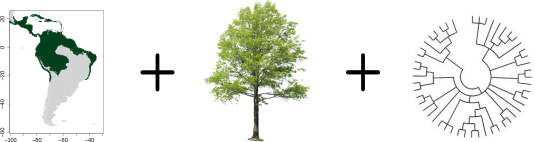
\includegraphics[width=0.5\textwidth]{./figures/Methods_figs.pdf}
%	%\includegraphics[scale=2]{./figures/Diversification_shifts_rate2.pdf}
%	\caption{}
%	\label{fig:methods}
%\end{figure}


\begin{tabular}{cp{0.3\textwidth}cp{0.4\textwidth}}

	\begin{minipage}{.15\textwidth}
		\includegraphics[width=\linewidth]{./figures/Range_maps_fig/Range_map_figure.pdf}
	\end{minipage} & 

\begin{itemize}
		\item BIEN 2.0 (range maps)
		\item 88,417 species
	\end{itemize} &

\begin{minipage}{.15\textwidth}
	\includegraphics[width=\linewidth]{./figures/tree_fig.png}
\end{minipage} &

\begin{itemize}
	\item BIEN 3.0 (trait observations)
	\item 8,820 species
\end{itemize} \\ 


\multicolumn{4}{c}{} \\

\multicolumn{4}{c}{} \\


\multicolumn{4}{c}{ \hspace{0.25\textwidth} \begin{minipage}{\textwidth}
		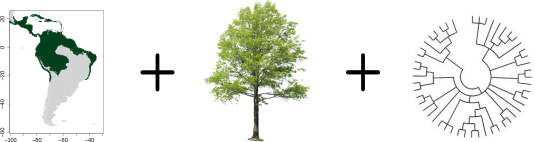
\includegraphics[width=0.5\linewidth]{./figures/Methods_figs.pdf} 
\end{minipage} } \\
\\ 
\multicolumn{4}{l}{ \hspace{0.15\textwidth} \textbf{7,842 species with complete trait information and range maps}}

\end{tabular}





\begin{figure}[h]
	\centering
	\includegraphics[width=\textwidth]{./figures/Trait_sampling}
	\caption{To estimate the functional trait space for each biome, we require complete trait data. For this reason, we phylogenetically imputed missing trait data using the R package ``Rphylopars'' v 0.2.9 (Goolsby et al., 2017) and the recently published phylogeny of seed plants by (Smith and Brown, 2018) as a baseline. }
	\label{fig:sampling}
\end{figure}



%\begin{figure}
%	\parbox{\LW}{\includegraphics[width=\linewidth]{./figures/Range_maps_fig/Range_map_figure.pdf}}%
%	\parbox{\LW}{\footnotesize BIEN 2.0 \\ 88,417 range maps of plant species}\qquad%
%	\parbox{\LW}{\includegraphics[width=0.7\linewidth]{./figures/tree_fig.png}}%
%	\parbox{\LW}{\footnotesize  BIEN 3.0 \\  8,820 species with trait observations \\ \tabitem Leaf phosphorus $[]$ (mg/g)}
%	\caption{}
%\end{figure}





	\end{block}

    \end{column}


    \begin{column}{\sepwid}\end{column}			% empty spacer column
    \begin{column}{\twocolwid}							% create a two-column-wide column and then we will split it up later

\begin{figure}[h]
	\centering
	\includegraphics[width=0.5\textwidth]{./figures/Figure1.pdf}
	~
	\includegraphics[width=0.3\textwidth]{./figures/Hypervolume_sp_sample_gaussian20perc.pdf}
	\caption{}
	\label{fig:map}
\end{figure}


		 \begin{block}{Results}


\begin{figure}[h]
	\centering
	\includegraphics[width=0.5\textwidth]{./figures/All_biomes_heatmap_logTraits.pdf}
	\caption{}
	\label{}
\end{figure}





		 \end{block}


 \end{column}



  \begin{column}{\sepwid}\end{column}			% empty spacer column
  \begin{column}{\onecolwid}



	\begin{figure}[h]
		\centering
		\includegraphics[width=0.6\textwidth]{./figures/heatmaps.pdf}
		\caption{}
		\label{}
	\end{figure}




			\begin{block}{Discussion}

      		\end{block}

      		\begin{block}{Next steps}

      		\end{block}



    \vskip2ex

          		\begin{block}{References}

		        \tiny{\begin{thebibliography}{99}



		        \end{thebibliography}}

			     \vspace{0.75in}

		 		\end{block}


      		\begin{block}{Acknowledgments}

      		\end{block}


    \vskip2ex

  \end{column}


  \begin{column}{\sepwid}\end{column}			% empty spacer column
 \end{columns}
\end{frame}
\end{document}
